% ============================================================
%  CHƯƠNG 5: CHAT & VIDEO CALL
%  Phụ trách: Nguyễn Tấn Khoa (MSSV: N22DCCN042)
%  Packages: ui/main/chat, ui/videocall,
%            services/MyFirebaseMessagingService,
%            services/CallForegroundService
%  Models:   data/model/chat/*, data/model/video/*,
%            data/model/notification/*
%  Local DB: data/local/entity/*, data/local/dao/ChatDao
%  Ghi chú: File này được \input{} từ main.tex
% ============================================================

\chapter{Chat và Gọi video}

% ============================================================
\section{Mô hình dữ liệu tổng thể}
% ============================================================

\subsection{Sơ đồ thực thể - quan hệ (ERD)}
Dữ liệu cục bộ chủ yếu phục vụ cho tính năng Chat nhằm hỗ trợ tối đa khả năng hoạt động ngoại tuyến (Offline/Caching) và tăng tốc độ kết xuất dữ liệu giao diện. Trong Room Database, mô hình quan hệ thực thể được thiết kế tập trung xung quanh các lớp Entity chính bao gồm:
\begin{itemize}
    \item \code{ConversationEntity}: Đại diện cho một cuộc hội thoại giữa hai người dùng (Room table: \code{conversations}). Lưu giữ ID hội thoại, tên đối tác chat (\code{partner\_name}), ảnh đại diện đối tác (\code{partner\_avatar}), nội dung tin nhắn cuối cùng để hiển thị trên danh sách (\code{last\_message}), số tin nhắn chưa đọc (\code{unread\_count}), và các mốc thời gian tạo/cập nhật hội thoại.
    \item \code{MessageEntity}: Đại diện cho từng tin nhắn riêng lẻ thuộc một hội thoại (Room table: \code{messages}). Chứa khóa chính \code{message\_id}, \code{conversation\_id} (có đánh chỉ mục \code{Index} để tối ưu hóa truy vấn), khóa ngoại người gửi \code{sender\_id}, nội dung văn bản tin nhắn \code{content}, loại tin nhắn \code{message\_type} (văn bản, hình ảnh, tập tin, hoặc lịch sử cuộc gọi), trạng thái tin nhắn \code{message\_status} (đã gửi, đã nhận, đã xem) và danh sách các tệp đính kèm đi kèm.
    \item \code{ConversationParticipantEntity}: Bảng trung gian xác định các thành viên tham gia cuộc trò chuyện (Room table: \code{conversation\_participants}). Liên kết khóa ngoại \code{conversation\_id} với bảng \code{conversations} bằng ràng buộc xóa lan tỏa (\code{onDelete = ForeignKey.CASCADE}).
    \item \code{MessageAttachmentEntity}: Lưu trữ siêu dữ liệu về các tệp tin hình ảnh/tài liệu đính kèm theo tin nhắn (Room table: \code{message\_attachments}), liên kết khóa ngoại \code{message\_id} đến bảng \code{messages} kèm ràng buộc xóa lan tỏa.
\end{itemize}

\subsection{Giao tiếp với Server}
Ứng dụng tương tác với máy chủ Node.js backend thông qua hai cơ chế giao tiếp bổ trợ nhau:
\begin{itemize}
    \item \tech{REST APIs (HTTP)}: Được triển khai thông qua thư viện \tech{Retrofit} kết hợp với adapter của \tech{RxJava 3} để trả về các luồng dữ liệu phản hồi kiểu bất đồng bộ như \code{Single<ResponseData<T>>}. Base URL của máy chủ được lưu trữ tập trung tại hằng số \code{Constants.BASE\_URL}, hỗ trợ tự động tuần tự hóa và giải tuần tự hóa JSON bằng \code{GsonConverterFactory}. Các endpoint chính bao gồm lấy danh sách hội thoại, gửi tin nhắn, tải tệp đính kèm, lấy cấu hình ICE và đăng ký token FCM.
    \item \tech{WebSockets (Socket.IO)}: Kết nối hai chiều liên tục sử dụng thư viện Socket.IO Client nhằm lắng nghe và phát các sự kiện thời gian thực (tin nhắn mới, trạng thái đã đọc, trạng thái gõ chữ, và tín hiệu gọi video WebRTC).
\end{itemize}

\textit{Đáp ứng CLO1: xây dựng hoàn chỉnh mô hình dữ liệu quan hệ cục bộ bằng Room DB và giao tiếp API đồng bộ sử dụng Retrofit và RxJava.}


% ============================================================
\section{Kiến trúc hệ thống Chat}
% ============================================================

\subsection{Tổng quan kiến trúc (Socket.IO + Room Database)}
Hệ thống tin nhắn áp dụng kiến trúc \tech{Clean Architecture} phối hợp với mô hình \tech{MVVM} và nguyên lý nguồn dữ liệu tin cậy duy nhất (Single Source of Truth - SSOT). Luồng luân chuyển dữ liệu tuân thủ nghiêm ngặt cơ chế một chiều:
Khi nhận được tin nhắn thời gian thực qua kênh kết nối Socket.IO hoặc khi tải lịch sử chat qua API REST, dữ liệu luôn được ghi trực tiếp vào Room Database cục bộ trước tiên thông qua \code{ChatDao}. Tầng giao diện (UI) không nhận dữ liệu trực tiếp từ API hay Socket mà luôn quan sát (observe) các luồng dữ liệu phản hồi liên tục \code{Flowable<List<MessageEntity>>} phát ra từ Room DB. Nhờ đó, bất kỳ thay đổi nào trong cơ sở dữ liệu cục bộ đều tự động phản chiếu lên màn hình trò chuyện ngay lập tức mà không gây giật lag UI.

\subsection{Mô hình dữ liệu cục bộ (ConversationEntity, MessageEntity)}
Các thực thể dữ liệu cục bộ được tối ưu hóa về mặt lưu trữ để phục vụ tính năng tìm kiếm và sắp xếp. Bảng \code{messages} sử dụng thuộc tính \code{indices} để đánh chỉ mục cho cột \code{conversation\_id} và \code{sender\_id}, giúp đẩy nhanh thời gian tải các tin nhắn của một phòng chat cụ thể. Các Attachments đính kèm trong \code{MessageEntity} được xử lý chuyển đổi kiểu dữ liệu (Type Converters) thông qua Gson để chuyển đổi qua lại giữa chuỗi JSON thô trong SQLite và đối tượng Java \code{List<AttachmentDto>} trên bộ nhớ RAM.

\subsection{Đồng bộ dữ liệu giữa Server và Local DB}
Để giải quyết bài toán mất mát tin nhắn khi người dùng ngoại tuyến (Offline) hoặc khi ứng dụng bị tắt hoàn toàn, hệ thống triển khai cơ chế đồng bộ hóa bắt tay (Handshake Synchronization) ngay khi kết nối Socket.IO được thiết lập lại.
Quy trình thực hiện bao gồm việc client truy vấn mốc thời gian của tin nhắn mới nhất có trong cơ sở dữ liệu Room DB cục bộ, sau đó gửi mốc thời gian này lên API \code{api/chat/messages/sync}. Server sẽ quét các tin nhắn mới phát sinh sau mốc thời gian đó và trả về danh sách đồng bộ. Client thực hiện chèn hàng loạt (bulk insert) vào local Room DB để khôi phục toàn vẹn dữ liệu.

Đoạn mã trích xuất luồng đồng bộ tin nhắn lỡ khi ứng dụng kết nối lại mạng được minh họa dưới đây:
\begin{lstlisting}[language=Java, caption=Đồng bộ tin nhắn lỡ khi kết nối lại mạng trong ChatRepository.java]
public Completable syncMissedMessages() {
    return Single.fromCallable(() -> {
        Date latestDate = chatDao.getLatestMessageTimestampSync();
        return latestDate != null ? isoFormat.format(latestDate) : "1970-01-01T00:00:00.000Z";
    })
    .flatMap(since -> apiService.syncMissedMessages(since, 100))
    .flatMapCompletable(response -> {
        if (response == null || response.getData() == null) 
            return Completable.complete();
        List<MessageEntity> entities = mapDtoListToEntity(response.getData());
        return chatDao.insertMessages(entities)
            .andThen(syncConversationLastMessages(entities));
    });
}
\end{lstlisting}

\textit{Đáp ứng CLO2: áp dụng thành công kiến trúc dữ liệu SSOT kết hợp Room DB và RxJava, đảm bảo khả năng đồng bộ hóa dữ liệu ngoại tuyến ổn định.}


% ============================================================
\section{Danh sách hội thoại}
% ============================================================

\subsection{Hiển thị danh sách cuộc trò chuyện}
\textbf{Yêu cầu chức năng:} Hiển thị danh sách các cuộc trò chuyện đang có của người dùng hiện tại, sắp xếp theo thời gian tin nhắn mới nhất giảm dần. Mỗi dòng hiển thị avatar đối tác, họ tên, nội dung tin nhắn cuối cùng (hoặc nhãn text thể hiện hình ảnh/cuộc gọi), thời điểm cập nhật và số lượng tin nhắn chưa đọc. Khi nhấn vào dòng hội thoại, ứng dụng chuyển sang màn hình chi tiết chat.

\textbf{Thiết kế giao diện:} Layout \code{fragment\_chat\_list.xml} chứa một \code{RecyclerView} làm trung tâm hiển thị danh sách cuộc trò chuyện, sử dụng \code{LinearLayoutManager} dọc. Giao diện mỗi hàng hội thoại (\code{item\_conversation.xml}) sử dụng \code{ShapeableImageView} bo tròn hiển thị ảnh đại diện, tích hợp thư viện \tech{Glide} để tải ảnh bất đồng bộ từ API file của server, cùng các thành phần \code{TextView} hiển thị tên đối tác và tin nhắn cuối.

\textbf{Luồng xử lý:}
\begin{enumerate}
    \item \code{ChatListFragment} được tạo, Hilt tiêm vào \code{ChatListViewModel}.
    \item ViewModel đăng ký nhận dữ liệu từ phương thức \code{observeConversations()} của \code{ChatRepository}.
    \item Repository trả về luồng dữ liệu \code{Flowable} liên kết trực tiếp với câu query Room Database của \code{ChatDao}.
    \item Khi có dữ liệu mới phát ra, \code{ConversationAdapter} nhận danh sách, tính toán thay đổi và gọi \code{notifyDataSetChanged()} để kết xuất lại.
    \item Người dùng nhấn vào một cuộc hội thoại, Fragment kích hoạt điều hướng (Navigation Component) sang \code{ChatFragment} truyền kèm tham số \code{conversationId}.
\end{enumerate}

\textbf{Triển khai trên Android:}
\begin{itemize}
    \item Lớp giao diện: \code{ChatListFragment} (giao diện danh sách), \code{ConversationAdapter} (kết nối dữ liệu).
    \item Lớp xử lý logic: \code{ChatListViewModel} kết nối với \code{ChatRepository}.
    \item API sử dụng: \code{GET api/chat/conversations} trả về danh sách \code{ConversationDto} chứa thông tin các participants để ánh xạ ngược lại tên người nhận.
\end{itemize}

\subsection{Huy hiệu tin nhắn chưa đọc (Unread Badge)}
\textbf{Yêu cầu chức năng:} Hiển thị một huy hiệu màu đỏ nổi bật chứa số lượng tin nhắn chưa đọc trên mỗi dòng hội thoại và bôi đậm tên đối tác cùng nội dung tin nhắn cuối cùng để người dùng dễ nhận biết cuộc trò chuyện có tin nhắn mới. Huy hiệu này phải tự biến mất và chữ hết bôi đậm ngay khi người dùng bấm mở phòng chat đó để xem tin nhắn.

\textbf{Thiết kế giao diện:} Sử dụng widget \code{TextView} (có ID là \code{badgeUnread}) để hiển thị số lượng tin nhắn chưa đọc. Trạng thái unread được thể hiện qua thuộc tính bôi đậm (\code{Typeface.BOLD}) và đổi màu chữ thành đen (\code{Color.BLACK}) trên các trường \code{tvName} và \code{tvLastMessage} trong layout dòng hội thoại \code{item\_conversation.xml}.

\textbf{Luồng xử lý:} Để đảm bảo tính đồng bộ và tránh sai lệch, số lượng tin nhắn chưa đọc được tính toán động (dynamic projection) thông qua câu truy vấn Room Database bằng cách đếm số tin nhắn thuộc hội thoại có trạng thái khác đã xem (\code{message\_status = 'SENT'}) và không phải do chính mình gửi (\code{sender\_id != :currentUserId}). Khi người dùng mở phòng chat, repository phát lệnh gọi API \code{POST api/chat/messages/read} và gửi sự kiện socket \code{message:read} để chuyển trạng thái tin nhắn về \code{READ}. Room Database tự động phát hiện thay đổi và kích hoạt tính toán lại \code{unread\_count}, tự động cập nhật ẩn badge và bỏ bôi đậm giao diện.

\textbf{Triển khai trên Android:} Thực thể giao diện \code{ConversationUIModel.java} chứa đối tượng \code{ConversationEntity} lồng kèm thuộc tính \code{lastMessageSenderId} và \code{lastMessageStatus}. Trong phương thức \code{onBindViewHolder} của \code{ConversationAdapter.java}, adapter kiểm tra biến đếm \code{conversation.unreadCount > 0} để bật/tắt \code{badgeUnread} (\code{View.VISIBLE} hoặc \code{View.GONE}) và highlight font chữ.

\subsection{Tìm kiếm hội thoại}
\textbf{Yêu cầu chức năng:} Cho phép người dùng tìm kiếm nhanh cuộc hội thoại theo tên đối tác bằng cách nhập từ khóa vào ô tìm kiếm nằm ở phía trên danh sách tin nhắn.

\textbf{Thiết kế giao diện:} Ô tìm kiếm sử dụng widget \code{EditText} (có ID là \code{etSearch}) được nhúng trong layout \code{fragment\_chat\_list.xml}. Ô này được trang bị icon kính lúp (\code{ic\_search}) và gợi ý văn bản để người dùng biết chức năng tìm kiếm.

\textbf{Luồng xử lý:} 
\begin{enumerate}
    \item Người dùng nhập từ khóa tìm kiếm vào ô nhập liệu \code{etSearch}.
    \item Giao diện lắng nghe sự kiện thay đổi văn bản qua \code{TextWatcher}. Nhằm tối ưu hiệu năng và hạn chế spam truy vấn, một cơ chế trì hoãn (Debounce) thời gian 400ms được thiết lập bằng \code{Handler} trước khi gọi hàm \code{search()} của \code{ChatListViewModel}.
    \item \code{ChatListViewModel} ghi nhận từ khóa, cập nhật biến \code{currentQuery}, đặt lại phân trang (\code{offset = 0}), và phát tín hiệu từ khóa mới qua đối tượng RxJava \code{BehaviorSubject} mang tên \code{querySubject}.
    \item Đồng thời, ViewModel thực hiện lệnh gọi API đồng bộ \code{fetchConversations()} từ máy chủ Node.js để tải về các kết quả hội thoại khớp với từ khóa và lưu vào local Room Database.
    \item Ở tầng truy vấn cơ sở dữ liệu, phương thức \code{observeConversations()} sử dụng toán tử RxJava \code{switchMap} để theo dõi \code{querySubject}. Nếu từ khóa rỗng, hệ thống trả về luồng quan sát toàn bộ hội thoại; ngược lại, hệ thống chuyển sang luồng quan sát lọc \code{observeConversationsFiltered(query)} liên kết trực tiếp với câu truy vấn Room Database của \code{ChatDao}.
\end{enumerate}

\textbf{Triển khai trên Android:} 
\begin{itemize}
    \item Lớp giao diện: \code{ChatListFragment.java} lắng nghe thay đổi văn bản và cập nhật LiveData kết quả lên adapter.
    \item Lớp xử lý logic và dữ liệu: \code{ChatListViewModel.java} quản lý trạng thái tìm kiếm và luồng dữ liệu RxJava; \code{ChatRepository.java} điều phối API đồng bộ và kết xuất database.
    \item Truy vấn Room DB: Phương thức \code{getConversationsWithStatusFiltered()} trong \code{ChatDao.java} thực hiện truy vấn SQL với từ khóa được định dạng bằng mệnh đề \code{LIKE} (\code{c.partner\_name LIKE :query}) để trích xuất các bản ghi trùng khớp theo thời gian thực từ bảng \code{conversations}.
\end{itemize}

\textit{Đáp ứng CLO2: xây dựng hoàn chỉnh giao diện danh sách hội thoại tương tác mượt mà, sử dụng RecyclerView, Glide, EditText và xử lý unread badge tự động.}






% ============================================================
\section{Nhắn tin thời gian thực}
% ============================================================

\subsection{Gửi và nhận tin nhắn văn bản}
\textbf{Yêu cầu chức năng:} Hỗ trợ gửi tin nhắn văn bản tức thời đến đối tác chat. Tin nhắn hiển thị trên khung bong bóng chat kèm thời gian gửi.

\textbf{Thiết kế giao diện:} Bong bóng chat sử dụng \code{RecyclerView} kết hợp với \code{ChatAdapter.java}. Giao diện áp dụng cơ chế thiết kế Multi-ViewType để hiển thị tin nhắn của người gửi ở lề phải (màu nền xanh dương nhạt hoặc xám đậm) và tin nhắn người nhận ở lề trái (màu trắng hoặc xám nhạt kèm avatar đối phương).

Đoạn mã cài đặt việc phân định ViewType được trình bày dưới đây:
\begin{lstlisting}[language=Java, caption=Phân chia Multi-ViewType trong ChatAdapter.java]
@Override
public int getItemViewType(int position) {
    MessageEntity message = getItem(position);
    boolean isSent = message.senderId == currentUserId;
    if (MessageType.IMAGE.equals(message.messageType)) {
        return isSent ? VIEW_TYPE_IMAGE_SENT : VIEW_TYPE_IMAGE_RECEIVED;
    } else if (MessageType.CALL.equals(message.messageType)) {
        return isSent ? VIEW_TYPE_CALL_SENT : VIEW_TYPE_CALL_RECEIVED;
    } else {
        return isSent ? VIEW_TYPE_TEXT_SENT : VIEW_TYPE_TEXT_RECEIVED;
    }
}
\end{lstlisting}

\textbf{Luồng xử lý:} Để tạo cảm giác phản hồi ngay lập tức (Optimistic UI updates), quy trình gửi tin được thiết kế như sau:
\begin{enumerate}
    \item Người dùng gõ tin nhắn và nhấn gửi.
    \item Client khởi tạo một đối tượng \code{MessageEntity} tạm thời có khóa chính là một số âm cực lớn (tính theo timestamp âm) mang trạng thái \code{MessageStatus.SENT}.
    \item Đối tượng tạm này được insert ngay lập tức vào Room DB. RecyclerView observe DB tự động vẽ lại tin nhắn này trên màn hình.
    \item Cùng lúc, ứng dụng kích hoạt lệnh gọi Retrofit API \code{POST api/chat/conversations/{id}/messages}.
    \item Nếu API thành công, máy chủ trả về \code{MessageDto} chứa ID chính thức dương ($>0$). Repository cập nhật Room DB để chèn tin nhắn chính thức và gỡ bỏ tin nhắn tạm bằng phương thức \code{softDeleteMessage}.
    \item Nếu API lỗi, trạng thái tin nhắn tạm được cập nhật thành \code{MessageStatus.ERROR} hiển thị dấu chấm than đỏ cảnh báo người dùng.
\end{enumerate}

\textbf{Triển khai trên Android:} Triển khai trong \code{ChatFragment}, \code{ChatViewModel} kết nối qua \code{ChatRepository} và \code{ChatDao}.

\subsection{Gửi ảnh đính kèm}
\textbf{Yêu cầu chức năng:} Người dùng có thể đính kèm và gửi hình ảnh được chọn từ thư viện điện thoại của họ vào phòng chat.

\textbf{Thiết kế giao diện:} Bong bóng chat hình ảnh sử dụng layout phẳng chuyên biệt \code{item\_chat\_image\_sent.xml} (cho ảnh gửi đi) và \code{item\_chat\_image\_received.xml} (cho ảnh nhận về) chứa thành phần \code{ImageView}. Sử dụng thư viện \tech{GlideApp} để tải ảnh bất đồng bộ từ URL, cấu hình tự động cache và hiển thị ảnh mượt mà, tối ưu RAM.

\textbf{Luồng xử lý:} Khi người dùng chọn ảnh, ứng dụng nhận \code{Uri}. ViewModel hiển thị trạng thái đang tải lên (\code{Resource.loading()}). Tại \code{ChatRepository.uploadMediaAndSendMessage()}, ứng dụng mở \code{InputStream} để sao chép dữ liệu byte từ Uri vào một tệp tạm thời trong thư mục cache (\code{context.getCacheDir()}), định danh định dạng (.png/.jpg). Sau đó, tệp tạm được gửi đi dưới dạng \code{MultipartBody.Part} thông qua API \code{POST api/chat/conversations/{id}/files}. Khi API trả về \code{MessageDto} chứa thông tin hình ảnh tải lên thành công, client xóa tệp tạm, insert thực thể chính thức vào Room DB và phát tín hiệu Socket.IO thông báo cho đối phương.

\textbf{Triển khai trên Android:} Sử dụng \code{ActivityResultContracts.GetContent()} với MIME filter là \code{image/*} trong \code{ChatFragment.java} để mở Gallery hệ thống. Logic tải lên được thực hiện trong \code{ChatViewModel.java} (phương thức \code{sendImage()}) kết hợp với phương thức \code{uploadMediaAndSendMessage()} của \code{ChatRepository.java} trên luồng background qua \code{Schedulers.io()}.

\subsection{Trạng thái tin nhắn (Sent / Delivered / Read)}
\textbf{Yêu cầu chức năng:} Cho phép theo dõi tiến trình gửi và nhận của tin nhắn gần nhất trong cuộc trò chuyện để biết tin nhắn đã được máy chủ tiếp nhận (\screen{Đã gửi}), đã nhận bên máy đối phương (\screen{Đã nhận}), đối phương đã mở xem (\screen{Đã xem}) hoặc gặp lỗi đường truyền (\screen{Lỗi}).

\textbf{Thiết kế giao diện:} Để tối ưu hóa giao diện và tránh gây rối mắt, trạng thái tin nhắn được ghép trực tiếp dưới dạng chuỗi văn bản (ví dụ: \screen{10:30 • Đã xem}) hiển thị tại thành phần \code{TextView} đại diện cho thời gian gửi (\code{tvTime}). Trạng thái này **chỉ hiển thị duy nhất** cho tin nhắn cuối cùng (last message) trong danh sách cuộc trò chuyện.

\textbf{Luồng xử lý:} Khi người dùng gửi tin, trạng thái mặc định được lưu cục bộ trong Room DB là \code{SENT} (\screen{Đã gửi}). Khi server hoặc đối phương phản hồi nhận/xem qua sự kiện socket \code{message:read} hoặc \code{message:delivered}, repository cập nhật trạng thái cột \code{message\_status} của tin nhắn tương ứng trong Room DB thành \code{READ} hoặc \code{DELIVERED}. UI observe sự thay đổi này và tự động vẽ lại.

\textbf{Triển khai trên Android:} Triển khai logic trong phương thức \code{onBindViewHolder} của \code{ChatAdapter.java}. Adapter kiểm tra vị trí tin nhắn xem có phải là tin cuối cùng trong danh sách hay không (\code{position == getItemCount() - 1}). Nếu đúng, nó bóc tách chuỗi \code{message.messageStatus} bằng cấu trúc \code{switch-case} để nối thêm văn bản trạng thái tương ứng vào trường \code{tvTime}. Nếu trạng thái là \code{ERROR}, màu chữ được đặt thành đỏ (\code{\#F44336}), ngược lại giữ màu xám mặc định (\code{\#888888}).

\subsection{Đánh dấu đã đọc (Mark as Read)}
\textbf{Yêu cầu chức năng:} Khi người dùng mở phòng chat, toàn bộ tin nhắn chưa đọc từ đối phương sẽ được đổi trạng thái thành đã đọc trên máy chủ.

\textbf{Luồng xử lý:} Khi \code{ChatFragment} tải danh sách tin nhắn từ Room DB, ViewModel quét toàn bộ danh sách tìm những ID tin nhắn thoả mãn hai điều kiện: được gửi bởi đối phương và trạng thái hiện tại khác \code{READ}. ViewModel gọi hàm \code{markMessagesAsRead()} đẩy mảng ID này lên API và đồng thời phát tín hiệu socket \code{message:read} đi.

\begin{figure}[H]
    \centering
    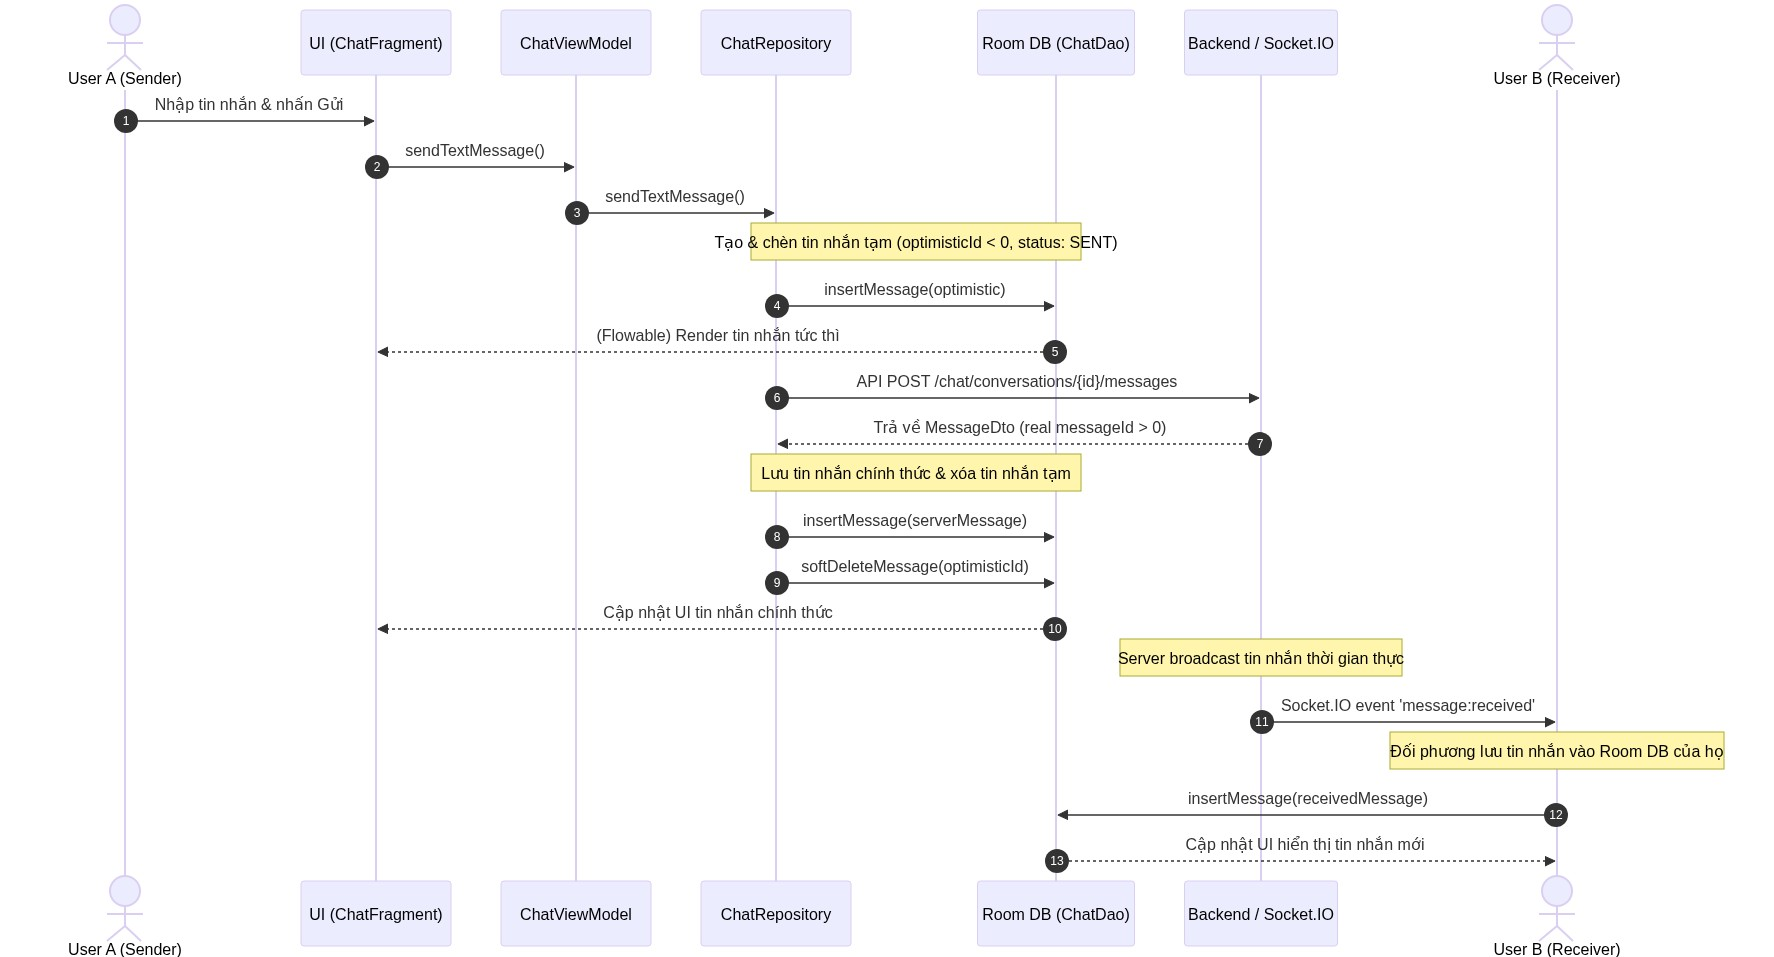
\includegraphics[width=0.85\textwidth]{images/outputs/c5_chat_flow.png}
    \caption{Sơ đồ luồng gửi và đồng bộ hóa tin nhắn thời gian thực}
    \label{fig:c5_chat_flow}
\end{figure}

\textit{Đáp ứng CLO2: cài đặt hoàn chỉnh tính năng chat thời gian thực sử dụng Socket.IO, Multi-ViewType RecyclerView, Glide load ảnh, cơ chế Optimistic UI và xử lý file đính kèm đa phương tiện.}


% ============================================================
\section{Thông báo đẩy (Push Notification)}
% ============================================================

\subsection{Tích hợp Firebase Cloud Messaging (FCM)}
Để giải quyết bài toán thông báo khi người dùng đã tắt hoặc đóng hoàn toàn ứng dụng (Killed), hệ thống tích hợp giải pháp thông báo đẩy Firebase Cloud Messaging (FCM) làm kênh dự phòng thụ động. Khi người dùng offline (không giữ kết nối Socket.IO), máy chủ Node.js Backend sẽ gửi yêu cầu push notification đến Google FCM Server để bắn tin nhắn/cuộc gọi đánh thức tiến trình nền của thiết bị nhận. Ngược lại, nếu người dùng đang online (ứng dụng đang chạy/mở), tin nhắn/cuộc gọi được phân phối trực tiếp qua Socket.IO với độ trễ tối thiểu, bypass hoàn toàn dịch vụ FCM để giảm tải hệ thống.

\subsection{Xử lý thông báo khi app ở foreground / background}
\textbf{Ứng dụng ở Foreground (Đang mở):} Thiết kế thông báo nội bộ (In-app Banner) thay thế hoàn toàn cho thông báo hệ thống của FCM. Khi có tin nhắn đến từ một cuộc trò chuyện khác qua Socket.IO (\code{activeConversationId != incomingId}), \code{ChatRepository} đẩy một sự kiện \code{InAppNotificationEvent} qua RxJava. \code{MainActivity} quan sát sự kiện này và kết xuất giao diện biểu ngữ trượt (\code{inAppNotificationBanner}) từ mép trên màn hình xuống (từ vị trí \code{-300f} về \code{0f} với thời gian 300ms bằng \code{DecelerateInterpolator}), tự động ẩn sau 4 giây. Người dùng nhấn vào biểu ngữ sẽ kích hoạt \code{navController.navigate} chuyển thẳng đến phòng chat chi tiết tương ứng.

\textbf{Ứng dụng ở trạng thái bị tắt hoàn toàn (Killed):} Khi có tin nhắn mới, Google FCM Server gửi Data-only payload đến thiết bị nhận. Tiến trình nền được đánh thức và phương thức \code{onMessageReceived()} của \code{MyFirebaseMessagingService.java} tiếp nhận payload, trích xuất dữ liệu rồi dựng một đối tượng \code{PendingIntent} bảo mật cao hỗ trợ cờ \code{FLAG\_UPDATE\_CURRENT | FLAG\_IMMUTABLE} trỏ đến \code{MainActivity}. Khi người dùng chạm vào thông báo nổi Heads-up trên thanh Notification bar, Intent kích hoạt bóc tách tham số và tự động dẫn người dùng trực tiếp vào phòng chat detail tương ứng.

Đoạn mã khởi tạo intent điều hướng trực tiếp được cài đặt như sau:
\begin{lstlisting}[language=Java, caption=Tạo PendingIntent điều hướng chat trong MyFirebaseMessagingService.java]
Intent intent = new Intent(this, MainActivity.class);
intent.putExtra("conversationId", conversationIdStr);
intent.addFlags(Intent.FLAG_ACTIVITY_NEW_TASK | Intent.FLAG_ACTIVITY_CLEAR_TOP);

PendingIntent pendingIntent = PendingIntent.getActivity(
    this, 
    (int) conversationId, 
    intent, 
    PendingIntent.FLAG_UPDATE_CURRENT | PendingIntent.FLAG_IMMUTABLE
);
\end{lstlisting}

\subsection{Lưu token FCM lên Server}
Để định danh thiết bị nhận thông báo đẩy, ứng dụng thực hiện lấy token FCM duy nhất từ Firebase SDK khi khởi động.
Token này được lưu trữ tạm thời tại local thông qua \code{SessionManager}. Khi người dùng đăng nhập thành công, token này được gửi đồng bộ lên API \code{POST api/notifications/tokens} để lưu trữ liên kết tài khoản trên máy chủ cơ sở dữ liệu. Khi người dùng đăng xuất (Logout), ứng dụng phát lệnh gọi API hủy liên kết token này nhằm đảm bảo tính bảo mật, ngăn chặn việc nhận thông báo của tài khoản cũ trên thiết bị.

\textit{Đáp ứng CLO1 và CLO2: tích hợp thành công dịch vụ thông báo đẩy Google FCM, xây dựng cơ chế xử lý notification thông minh giữa foreground/background và deep-link điều hướng màn hình.}


% ============================================================
\section{Gọi video (WebRTC)}
% ============================================================

\subsection{Tổng quan công nghệ WebRTC và Coturn STUN/TURN}
Để thiết lập cuộc gọi hình ảnh trực tiếp chất lượng cao với độ trễ thấp giữa hai thiết bị (P2P), ứng dụng sử dụng công nghệ truyền thông gian thực \tech{WebRTC} (thư viện \code{io.github.webrtc-sdk:android}).
Tuy nhiên, trong môi trường internet thực tế, các thiết bị thường nằm sau các lớp tường lửa hoặc hệ thống dịch địa chỉ mạng (NAT) phức tạp khiến chúng không thể kết nối trực tiếp. Ứng dụng tích hợp hệ thống máy chủ phụ trợ \tech{Coturn} cung cấp hai dịch vụ thiết yếu:
\begin{itemize}
    \item \tech{STUN (Session Traversal Utilities for NAT)}: Giúp thiết bị tự xác định địa chỉ IP công cộng và cổng của chính mình.
    \item \tech{TURN (Traversal Using Relays around NAT)}: Đóng vai trò máy chủ trung gian chuyển tiếp (relay) toàn bộ gói tin media (hình ảnh, âm thanh) giữa hai thiết bị khi mọi nỗ lực kết nối ngang hàng trực tiếp (P2P) thất bại.
\end{itemize}
Cấu hình danh sách các máy chủ STUN/TURN được lấy động từ API REST \code{api/video-call/ice-config} trước khi bắt đầu đàm phán cuộc gọi.

\subsection{Luồng thiết lập cuộc gọi (Signaling qua Socket.IO)}
Quá trình đàm phán kết nối WebRTC (Signaling) được thực hiện thông qua kênh WebSockets thời gian thực của Socket.IO, tuân thủ các bước đàm phán tuần tự (xem Sơ đồ Hình~\ref{fig:c5_call_flow}):
\begin{enumerate}
    \item Người gọi (Caller) lấy danh sách ICE Servers và gửi sự kiện socket \code{video:call:createRoom} truyền kèm calleeId.
    \item Server tạo mã phòng gọi duy nhất (\code{roomId}) lưu trữ vào Redis và phát tín hiệu đánh thức Callee (gửi socket trực tiếp nếu callee online hoặc đẩy FCM cuộc gọi nếu offline).
    \item Thiết bị Callee mở màn hình \code{IncomingCallActivity}. Khi nhấn Chấp nhận, Callee lấy danh sách ICE Servers và gửi sự kiện socket \code{video:call:accepted}.
    \item Cả hai thiết bị cùng gửi sự kiện socket \code{video:call:joinRoom} để kết nối chung vào phòng.
    \item Caller tạo ra một bản mô tả phiên kết nối \code{SDP Offer}, thiết lập cấu hình cục bộ và gửi sang Callee.
    \item Callee nhận được SDP Offer, ghi nhận cấu hình từ Caller, sinh ra bản mô tả phản hồi \code{SDP Answer} và gửi ngược lại Caller.
    \item Hai thiết bị trao đổi liên tục các gói tin ứng viên mạng \code{ICE Candidates} (gói tin đục lỗ NAT STUN/TURN) để dò tìm đường truyền tốt nhất.
    \item Khi tìm được đường đi, kênh kết nối P2P media trực tiếp được thiết lập thành công.
\end{enumerate}

\begin{figure}[H]
    \centering
    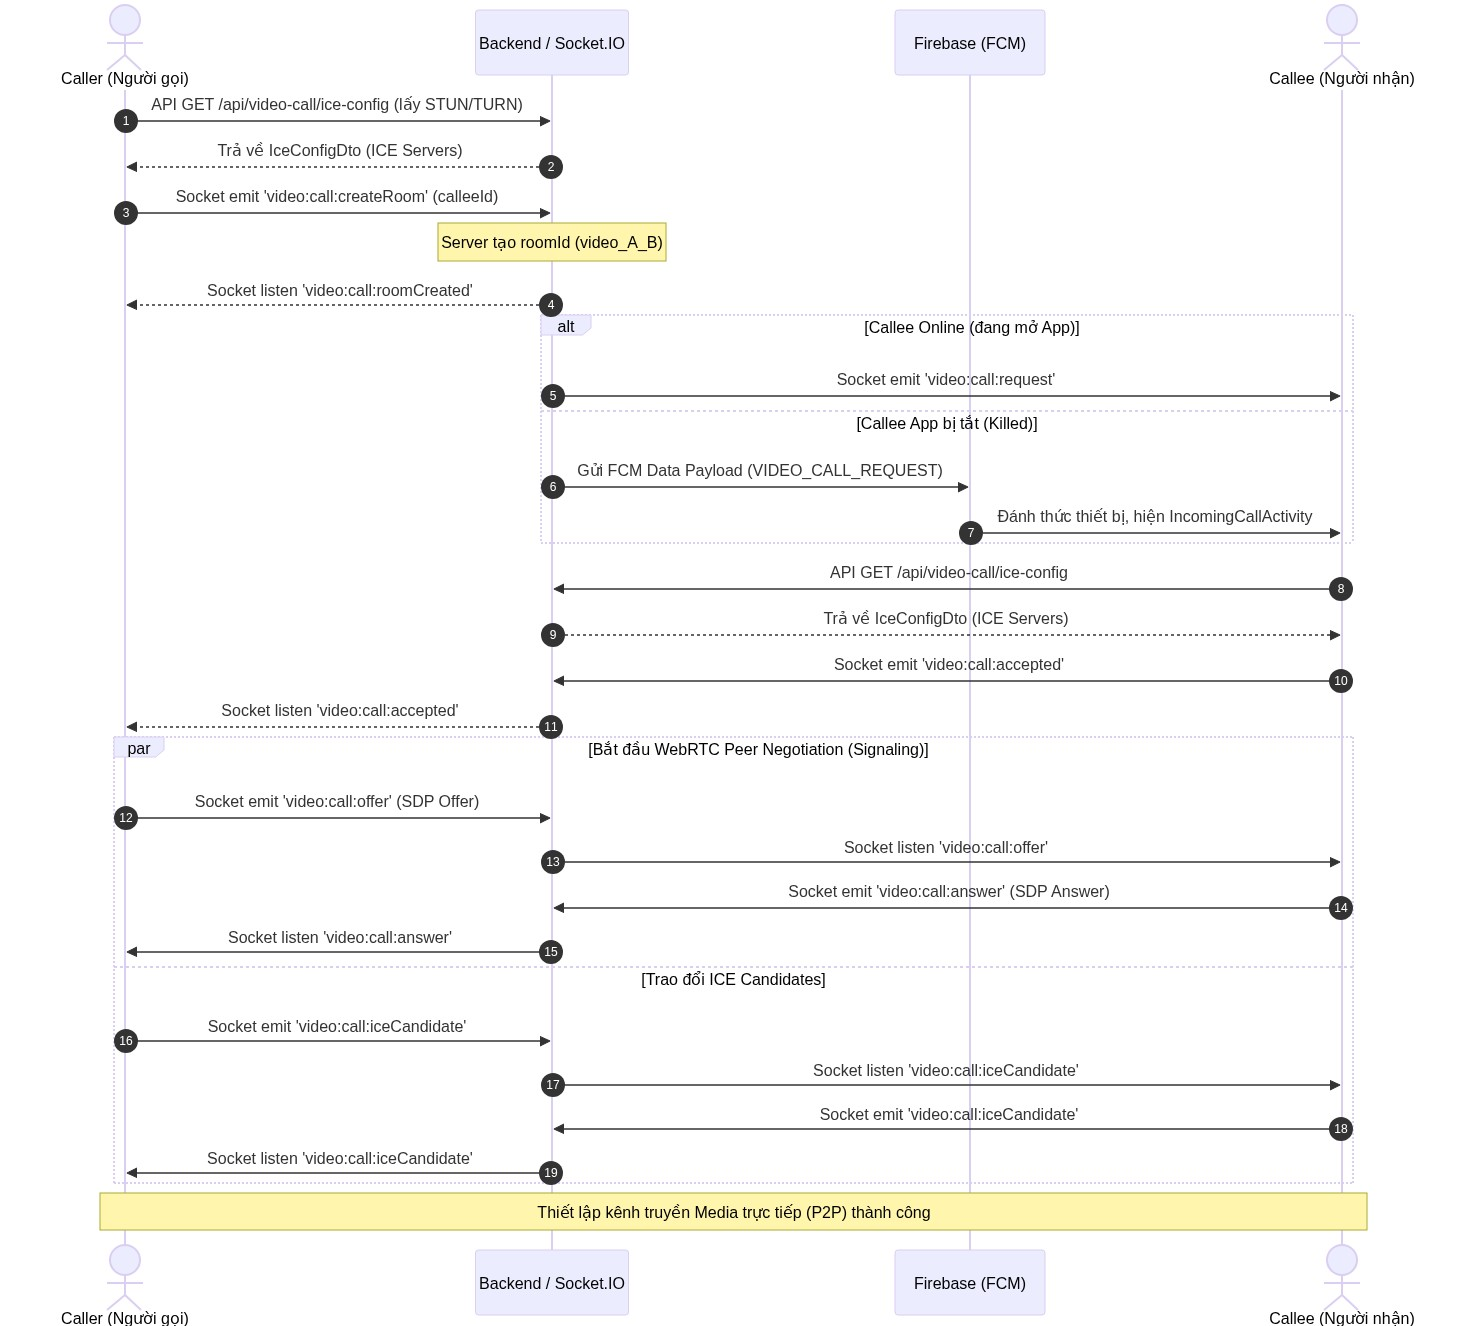
\includegraphics[width=0.85\textwidth]{images/outputs/c5_call_flow.png}
    \caption{Sơ đồ tuần tự quá trình đàm phán Signaling thiết lập cuộc gọi WebRTC}
    \label{fig:c5_call_flow}
\end{figure}

\subsection{Màn hình gọi đến (IncomingCallActivity)}
\textbf{Yêu cầu chức năng:} Hiển thị giao diện rung chuông toàn màn hình khi có cuộc gọi video đến, hiển thị tên và avatar người gọi kèm hai nút chức năng Chấp nhận và Từ chối. Giao diện phải hoạt động được ngay cả khi màn hình điện thoại đang khóa.

\textbf{Thiết kế giao diện:} Layout \code{activity\_incoming\_call.xml} sử dụng nền mờ kèm hình ảnh đại diện lớn của người gọi đặt ở trung tâm. Hai nút \code{fab\_accept} (màu xanh lá) và \code{fab\_decline} (màu đỏ) được đặt nổi bật phía dưới màn hình. Giao diện sử dụng \code{RingtoneManager} để phát nhạc chuông cuộc gọi và \code{Vibrator} tạo độ rung liên tục.

\textbf{Luồng xử lý:} Khi nhận được sự kiện gọi đến, dịch vụ nền kích hoạt màn hình \code{IncomingCallActivity}. Màn hình này cấu hình các cờ đặc biệt trỏ đến Window Manager bao gồm \code{setShowWhenLocked(true)} và \code{setTurnScreenOn(true)} để ép bật sáng màn hình điện thoại và đè lên trên lớp màn hình khóa bảo mật của thiết bị Android. Nếu sau 30 giây người dùng không tương tác, màn hình tự động phát sự kiện từ chối do timeout và đóng Activity.

\subsection{Màn hình gọi video (VideoCallActivity)}
\textbf{Yêu cầu chức năng:} Hiển thị luồng video thời gian thực từ camera của mình và camera của đối phương trong quá trình đàm thoại. Cung cấp các nút tương tác: bật/tắt camera, bật/tắt mic, chuyển đổi camera trước/sau, và cúp máy kết thúc cuộc gọi.

\textbf{Thiết kế giao diện:} Layout \code{activity\_video\_call.xml} chứa hai khung hình hiển thị video sử dụng thành phần \code{SurfaceViewRenderer} của thư viện WebRTC. Khung hình đối phương (\code{remoteVideoView}) hiển thị full-screen làm nền chính. Khung hình cá nhân (\code{localVideoView}) hiển thị trong một cửa sổ nhỏ đặt nổi góc trên bên phải màn hình. Thanh chức năng nằm ở cạnh dưới chứa các nút bật/tắt nhanh thiết bị phần cứng.

Đoạn mã cài đặt khởi tạo camera và hiển thị luồng stream nội bộ lên UI được minh họa dưới đây:
\begin{lstlisting}[language=Java, caption=Khởi tạo các thành phần render video WebRTC trên giao diện]
private void initWebRtc(IceConfigDto iceConfig) {
    // 1. Khoi tao cau hinh WebRtcManager cuc bo
    webRtcManager.init(iceConfig, roomId);

    // 2. Khoi tao Renderer hien thi Camera
    binding.localVideoView.init(webRtcManager.getEglContext(), null);
    binding.localVideoView.setEnableHardwareScaler(true);
    binding.localVideoView.setMirror(true);

    binding.remoteVideoView.init(webRtcManager.getEglContext(), null);
    binding.remoteVideoView.setEnableHardwareScaler(true);

    // 3. Dinh kem Local Stream de hien thi len UI
    if (webRtcManager.getLocalVideoTrack() != null) {
        webRtcManager.getLocalVideoTrack().addSink(binding.localVideoView);
    }
}
\end{lstlisting}

\textbf{Luồng xử lý:}
\begin{enumerate}
    \item \code{VideoCallActivity} mở ra sau khi bấm chấp nhận cuộc gọi.
    \item Hàm \code{initWebRtc()} được gọi thiết lập các thông số phần cứng camera/micro.
    \item Đối tượng \code{VideoTrack} thu tín hiệu từ camera trước của thiết bị truyền dữ liệu vào sink của \code{localVideoView}.
    \item Khi đàm phán thành công và nhận được remote track từ máy chủ, callback \code{onRemoteVideoTrackAdded()} được kích hoạt trên luồng UI để vẽ luồng video nhận được lên \code{remoteVideoView}.
    \item Khi người dùng tắt màn hình hoặc đóng cuộc gọi, hàm \code{onDestroy()} bắt buộc phải giải phóng tuần tự toàn bộ tài nguyên phần cứng để tránh lỗi rò rỉ bộ nhớ (memory leak).
\end{enumerate}

\subsection{Kết thúc và từ chối cuộc gọi}
Khi một trong hai bên nhấn nút Cúp máy, ứng dụng phát sự kiện socket \code{video:call:ended} và thực hiện giải phóng WebRTC Engine cục bộ.
Đối phương nhận được sự kiện socket kết thúc cuộc gọi sẽ tự động hiển thị thông báo cuộc gọi kết thúc và đóng màn hình trò chuyện lập tức. Khi kết thúc cuộc gọi, máy chủ tự động lưu trữ một tin nhắn chat lịch sử cuộc gọi hệ thống có kiểu \code{CALL} vào cơ sở dữ liệu để hiển thị trong phòng chat chi tiết (VD: \screen{Cuộc gọi thoại - 5:20} hoặc \screen{Cuộc gọi nhỡ}).

\textit{Đáp ứng CLO1 và CLO2: xây dựng hoàn chỉnh tính năng gọi video 1-1 phức tạp, tích hợp sâu kỹ thuật WebRTC, máy chủ NAT STUN/TURN, đàm phán Signaling qua socket và xử lý render camera hiệu suất cao.}


% ============================================================
\section{Dịch vụ nền cuộc gọi (CallForegroundService)}
% ============================================================

\subsection{Foreground Service và Notification khi đang gọi}
Để đảm bảo luồng hình ảnh và âm thanh cuộc gọi không bị hệ điều hành Android tự động tối ưu hóa giải phóng bộ nhớ (kill process) khi người dùng bấm nút Home ẩn ứng dụng để làm việc khác, ứng dụng xây dựng dịch vụ chạy nổi \code{CallForegroundService}.
Dịch vụ được cấu hình kiểu chuyên biệt \code{foregroundServiceType="phoneCall"} đáp ứng chuẩn bảo mật khắt khe của hệ điều hành từ Android 14+ trở lên. Khi cuộc gọi hoạt động, dịch vụ kích hoạt một thông báo treo (\code{startForeground}) hiển thị trạng thái \screen{Cuộc gọi đang diễn ra} kèm thời gian đàm thoại, ngăn chặn việc hệ thống thu hồi tài nguyên camera/micro.

\subsection{Xử lý cuộc gọi đến khi màn hình khóa}
Nhờ sự bổ trợ của Full-Screen Intent trong Notification Channel kết hợp với cơ chế giữ màn hình sáng (\code{WakeLock}), khi có thông báo cuộc gọi đẩy đến từ FCM lúc điện thoại đang ở chế độ ngủ sâu khóa màn hình, Android OS tự động ưu tiên cấp quyền khởi chạy trực tiếp cửa sổ giao diện của màn hình chờ cuộc gọi \code{IncomingCallActivity}. Người dùng có thể thực hiện thao tác Vuốt hoặc chạm để trả lời trực tiếp mà không cần mở khóa mật khẩu màn hình trước, đem lại trải nghiệm mượt mà giống như các ứng dụng đàm thoại chuyên nghiệp khác.

\textit{Đáp ứng CLO2: tối ưu hóa vòng đời ứng dụng chạy nền qua Android Foreground Service và xử lý tương tác cuộc gọi màn hình khóa mượt mà.}
